As we mentioned, GDSDA is a paradigm using GD for the SDA problem. In this section, we first give a brief review of GD. Then we show the process of GDSDA and demonstrate the reason why GDSDA can work for the SDA problem. Finally, we show the importance of the imitation parameter. 
\begin{figure}\label{fig:gd}
\centering
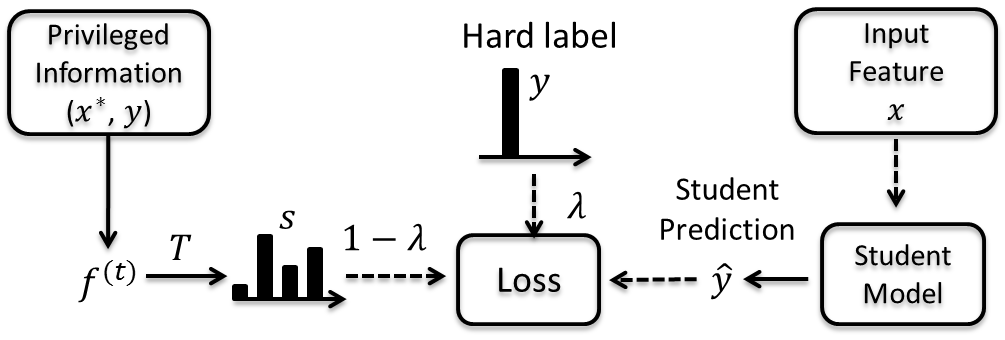
\includegraphics[scale=.35]{figure/GD.png}
\caption{Illustration of Generalized Distillation training process.}
\end{figure}
\subsection{An overview of Generalized Distillation and GDSDA}
%
%
%\textit{Distillation} \cite{hinton2015distilling} and \textit{Learning Using Privileged Information} (LUPI) \cite{vapnik2015learning} are two paradigms that enable machines to learn from other machines. Both methods address the problem of how to build a student model that can learn from the advanced teacher models. Recently, Lopez {et al.} \cite{lopez2015unifying} proposed a framework called \textit{generalized distillation} that unifies both methods and show that it can be applied in many scenarios.
{Generalized Distillation} can be considered as the hybrid of two famous learning paradigms \textit{Distillation} \cite{hinton2015distilling} and \textit{Learning Using Privileged Information} (LUPI) \cite{vapnik2015learning} .
In GD, the training data can be represented as a collection of the triples:
\[\{\left(x_1,x_1^*,y_1\right),\left(x_2,x_2^*,y_2\right) \dots \left(x_n,x_n^*,y_n\right)\}\]. 
$x^*$ is the privileged information for data $x$, which is only available in the training set and $y$ is the corresponding label. 
The process of generalized distillation is as follows: in step 1, a teacher model ${f}^{(t)}$ is trained using the input-output pairs $\{x^*_i,y_i\}_{i=1}^n$. In step 2, use ${f}^{(t)}$ to generate the soft label $s_i$ for each training example $x_i$ using the softmax function $\sigma$:
\begin{equation}\label{eq:softmax_T}
s_i=\sigma(f^{(t)}(x_i)/T)
\end{equation}
where $T$ is a hyperparameter called temperature to control the smoothness of the soft label. In step 3, learn the student ${f}^{(s)}$ from the pairs $\{\left(x_i,y_i\right),\left(x_i,s_i\right)\}_{i=1}^n$ using:
\begin{equation}\label{eq:distill}
\begin{aligned}
f^{(s)}=&\underset{f^{(s)} \in \mathcal{F}^{(s)}}{\arg \min}\frac{1}{n}\sum_{i=1}^{n}\bigg[\lambda\ell\left(y_i,\sigma(f^{(s)}(x_i))\right)+(1-\lambda)\ell\left(s_i,\sigma(f^{(s)}(x_i))\right)\bigg]\\
\end{aligned}
\end{equation}
Here, $\ell(\cdot,\cdot)$ is the loss function and $\lambda$ is the imitation parameter to balance the importance between the hard label $y_i$ and the soft label $s_i$.

